\documentclass[tikz,border=10pt]{standalone}
\usetikzlibrary{calc}
\begin{document}
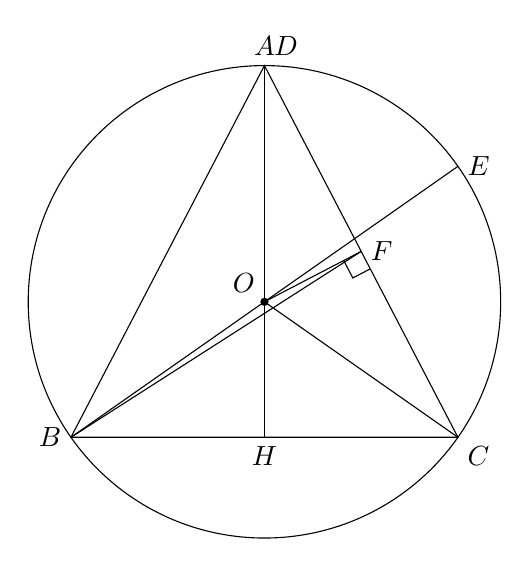
\begin{tikzpicture}[scale=1]
  % Circle center O and radius
  \coordinate (O) at (0,0);
  \def\r{3}
  % Points on circle
  \coordinate (A) at (90:\r);
  \coordinate (B) at (215:\r);
  \coordinate (C) at (325:\r);
  \coordinate (E) at (35:\r);
  % H midpoint of BC, D = intersection of AE and BC-line region
  \coordinate (H) at ($(B)!0.5!(C)$);
  % D is intersection of line AE with line AC
  \coordinate (D) at (intersection of A--E and B--C);
  % Actually D lies on AC; compute intersection of AE and AC
  \coordinate (D) at (intersection of A--E and A--C);
  % F foot of perpendicular from O to AC
  \coordinate (F) at ($(A)!(O)!(C)$);
  % Draw circle
  \draw (O) circle (\r);
  % Triangle and chords
  \draw (A) -- (B) -- (C) -- cycle;
  \draw (A) -- (H);
  \draw[dashed] (A) -- (O);
  \draw (O) -- (H);
  \draw (B) -- (E);
  \draw (O) -- (F);
  \draw (B) -- (F);
  \draw (O) -- (C);
  % Right angle mark at F
  \draw ($(F)!0.25cm!(O)$) -- ($($(F)!0.25cm!(O)$)!0.25cm!90:(O)$) -- ($(F)!0.25cm!(C)$);
  % Points
  \fill (O) circle (1.5pt);
  % Labels
  \node[above] at (A) {$A$};
  \node[left] at (B) {$B$};
  \node[below right] at (C) {$C$};
  \node[right] at (E) {$E$};
  \node[above right] at (D) {$D$};
  \node[above left] at (O) {$O$};
  \node[right] at (F) {$F$};
  \node[below] at (H) {$H$};
\end{tikzpicture}
\end{document}
